% Teorema: tabel nilai tempat + peraga lempeng
% Kompilasi: pdflatex nilai-tempat-tikz.tex
\documentclass[border=14pt]{standalone}
\usepackage{tikz}
\usepackage{amsmath}
\definecolor{bg}{HTML}{171D2B}
\definecolor{akun}{HTML}{F7B538}
\definecolor{garis}{HTML}{4B5563}
\definecolor{sel}{HTML}{232B3E}
\pagecolor{bg}
\color{white}
\begin{document}
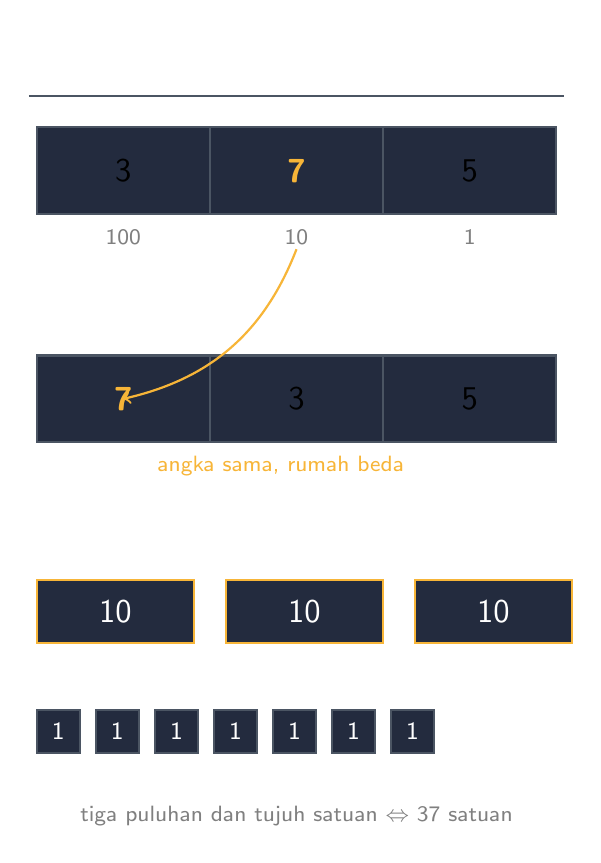
\begin{tikzpicture}[
  kotak/.style={draw=garis, fill=sel, thick, minimum width=2.2cm, minimum height=1.1cm},
  font=\sffamily\large
]
\def\cw{2.2}
\def\ch{1.1}

% ---------- Gambar 1: tabel nilai tempat ----------
\begin{scope}[yshift=0cm]
  % kepala kolom
  \foreach \i/\nama in {0/Ratusan, 1/Puluhan, 2/Satuan} {
    \node[white] at ({\i*\cw+\cw/2}, 0.55) {\textbf{\nama}};
  }
  \draw[garis, thick] (-0.1,-0.05) -- (3*\cw+0.1,-0.05);
  % baris bilangan 375
  \foreach \i/\t in {0/3, 1/{\textcolor{akun}{\textbf{7}}}, 2/5} {
    \node[kotak] at ({\i*\cw+\cw/2}, -1.0) {\t};
    \node[gray, font=\sffamily\footnotesize] at ({\i*\cw+\cw/2}, -1.85)
      {\pgfmathparse{int(100/10^\i)}\pgfmathresult};
  }
  % baris bilangan 735
  \begin{scope}[yshift=-2.9cm]
    \foreach \i/\t in {0/{\textcolor{akun}{\textbf{7}}}, 1/3, 2/5} {
      \node[kotak] at ({\i*\cw+\cw/2}, -1.0) {\t};
    }
  \end{scope}
  % panah penghubung kedua angka 7
  \draw[akun, thick, ->] ({1.5*\cw},-2.0) to[bend left=28] ({0.5*\cw},-3.9);
  \node[akun, font=\sffamily\footnotesize] at (3.1, -4.75) {angka sama, rumah beda};
\end{scope}

% ---------- Gambar 2: lempeng nilai tempat ----------
\begin{scope}[yshift=-7.0cm, xshift=0cm]
  \node[white] at (3.3, 1.5) {\textbf{Lempeng: $3\times10 + 7\times1 = 37$}};
  % 3 lempeng puluhan
  \foreach \i in {0,1,2} {
    \draw[fill=sel, draw=akun, thick] ({\i*2.4},0) rectangle ++(2.0,0.8);
    \node[white] at ({\i*2.4+1.0}, 0.4) {10};
  }
  % 7 lempeng satuan
  \foreach \i in {0,...,6} {
    \draw[fill=sel, draw=garis, thick] ({\i*0.75},-1.4) rectangle ++(0.55,0.55);
    \node[white, font=\sffamily\small] at ({\i*0.75+0.275}, -1.125) {1};
  }
  \node[gray, font=\sffamily\footnotesize] at (3.3, -2.2) {tiga puluhan dan tujuh satuan $\Leftrightarrow$ 37 satuan};
\end{scope}
\end{tikzpicture}
\end{document}
